\section{Konsept og spillutforming}\label{sec:konsept}

\subsection{Introduksjon: Garbage Alert}

			\begin{figure} [here]
				\begin{center}
					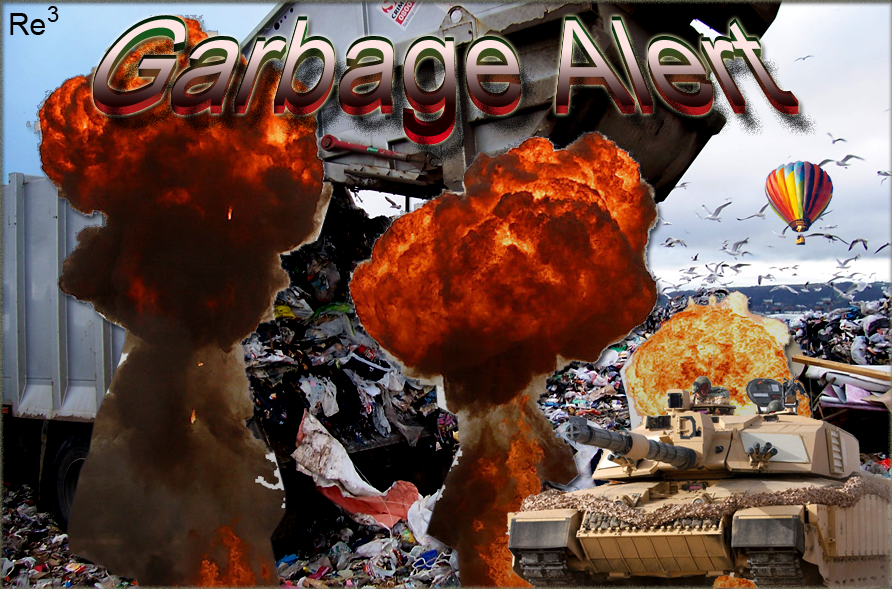
\includegraphics[scale=0.5]{images/splashscreen}
				\end{center}
			\caption{Garbage Alert splash screen}
		\end{figure}

Garbage Alert er strategispillet der du bestemmer verdens skjebne ved å gjenvinne og krige med søppel. Spillet har resirkulering i sentrum samtidige som det skal være et underholdende strategispill for deg mellom 9 og 99 år. 

Man starter på en øy overfyllt med søppel. Målet med spillet er å bli kvitt søppelet. Ved å gjenvinne avfallet får man ulike muligheter til å bombandere de andre spillerne, forsvare sin egen øy, for så å stå igjen som vinneren på en øy uten søppel, eller som eneste spiller i live.

Spillet er utviklet av en gruppe studenter på NTNU i faget Eksperter i Team. Spilldesignerne går under navnet Re3. Re3 består av Andreas Røysland Aarnes, Trond Kjetil Bremnes, Christian Aleksander Lysne, Kjetil Mehl og Ina Sander Pedersen.

Målet med dette avsnittet er å gi deg et innblikk i det utviklede spillkonseptet,
hvilke spillaspekter som er tatt med og spilldynamikken.


% This is a section where the definition of the game play is established.
% Definitions should include how a player wins, loses, passes levels and
% the main focus of the game play.
\subsection{Definisjoner}
Dette avsnittet forklare de grunnleggende definisjonene rundt Garbage
Alert. Definisjonene er i hovedsak sentrert rundt hvordan spilleren
oppfatter spillet~\cite{gameplay}.
\subsubsection{Oppstart}
Alle spillere starter med like forutsetninger. Hvordan spillet utvikler
seg kommer an på hvordan spillerene bruke ressursene som er gitt.
\subsubsection{Vinning}
En spiller har vunnet dersom alle de andre spillerene har mistet
gjenvinningsstasjonene sine, eller spilleren klarer å blit kvitt alt
søppelet på sin øy.
\subsubsection{Taping}
En spiller taper dersom gjenvinningsstajonen dens blir ødelagt. Spilleren
vil også tape dersom en annen spiller klarer å renske sin øy for søppel.


\subsection{Spilldynamikken}

Garbage Alert er i utgangspunktet et flerspiller sanntidsstrategispill, men det er også mulighet for å spille alene mot spillere med kunstig intelligens. 

Man starter spillet med en øy og følgende elementer:

\begin{itemize}
	\item Et resirkuleringssenter
	\item En våpenstasjon
	\item En forsvarssone
	\item 10 enheter med papp i inventaret
	\item 1000 enheter med søppel
	\item Muligheten til å gjenvinne papp fra søppelet. Gjenvinningsgraden er 10\%
	\item Muligheten til å bruke papp til å bygge våpen (papirfly) og forsvar (pappmur)
	\item Muligheten til å oppgradere gjenvinningsgraden til 20\%
	\item Muligheter for oppgraderinger av gjenvinningsstasjon slik at man også får gjenvinnet plast eller tre.
\end{itemize}

Jo flere typer ressurser man får gjenvinnet fra søppelet, jo flere muligheter har man for mer avanserte våpen, forsvar og oppgraderinger. Man starter med å kun gjenvinne papp. Figur XX viser mulighetene man har for å oppgradere resirkuleringssenteret slik at man får muligheten til å gjenvinne andre ressurser. For eksempel hvis man skal oppgradere til stål, må man først oppgradere til plast. For å oppgradere til titan kreves det at alle andre oppgraderinger allerede er utført. \\

	\begin{figure} [H]
				\begin{center}
					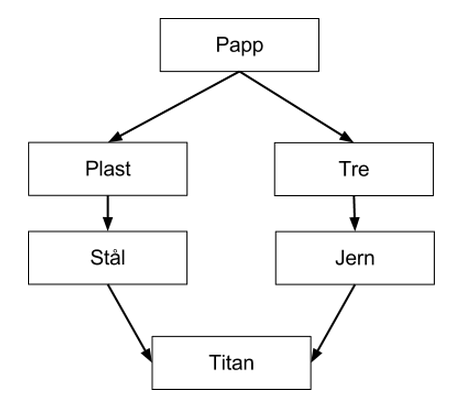
\includegraphics[scale=0.5]{images/oppgraderingstre}
				\end{center}
			\caption{Ressursoppgraderinger}
	\end{figure}
		
I tillegg til disse oppgraderingene har man også muligheten til å oppgradere gjenvinningseffektiviteten. Man har da følgende muligheter: \\

		\begin{figure} [H]
				\begin{center}
					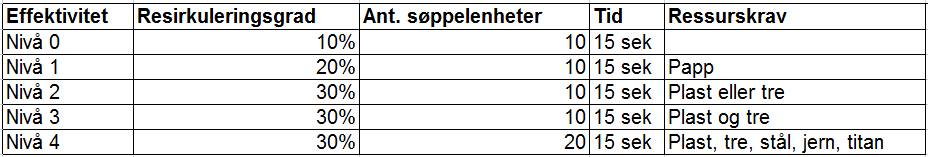
\includegraphics[scale=0.5]{images/effektivitet}
				\end{center}
			\caption{De ulike oppgraderingingene for effektivitet. Ved 10\% resirkuleringsgrad og 10 søppelenheter for man 1 enhet med ressurser per ressursoppgradering man har}
		\end{figure}


%tabellen virker ikke av en eller annen grunn.....må få det til å funke, bilde
%brukt i stedet, men det er litt feil...
%\begin{tabularx}{300pt}{| l | l | l | l | l |}
%\hline
%\bf{Effektivitet} & \bf{Resirkuleringsgrad} & \bf{Ant. søppelenheter} & \bf{Tid} & %\bf{Ressurskrav} \\
%\hline
%Nivå 0 & 10 & 10 & 15sek & Ingen  \\
%Nivå 1 & 20 & 10 & 15sek & Papp \\
%Nivå 2 & 30 & 10 & 15sek & Papp, og plast eller tre \\
%Nivå 3 & 30 & 20 & 15sek & Papp, plast, tre, stål, jern og titan \\
%\hline
%\end{tabularx}

%De sentrale spillelementene består av å samle inn søppel til resikulerings vil være samling, %ressursforvaltning, valg av våpen og forsvar, samt timing av våpenbruk. Spillinnholdet vil hovedsaklig være Pure Play (Usikker på dette innebærer det jeg tror), der målet er å få spilleren til å ha det gøy, men det vil også være elementer av realisme da det spilleren foretar seg vil virke inn på både lokalt og globalt miljø. Det vil være en lineær spillsekvens (Er usikker på denne fordi jeg ikke finner noen  spillsekvenstype som passer??) der spilleren får tilgang til nye våpentyper og forsvarsmuligheter etterhvert som krav for hver enkelt oppgradering er nådd. For at spillet skal få et lekent og fristende utseende har vi valgt en type tegneseriestil som vil gjøre nettopp dette. (Husker ikke om vi har vi diskutert dette, og hva vi kom fram til?)\\

%Spillbeskrivelse: Spillets sjanger er valgt til flerspiller sanntidsstrategi, men det vil også være mulighet for å spille alene mot computer. (Usikker på om vi ble enig om at dette skulle være mulig?) Viktige spillelementer vil være samling, ressursforvaltning, valg av våpen og forsvar, samt timing av våpenbruk. Spillinnholdet vil hovedsaklig være Pure Play (Usikker på dette innebærer det jeg tror), der målet er å få spilleren til å ha det gøy, men det vil også være elementer av realisme da det spilleren foretar seg vil virke inn på både lokalt og globalt miljø. Det vil være en lineær spillsekvens (Er usikker på denne fordi jeg ikke finner noen  spillsekvenstype som passer??) der spilleren får tilgang til nye våpentyper og forsvarsmuligheter etterhvert som krav for hver enkelt oppgradering er nådd. For at spillet skal få et lekent og fristende utseende har vi valgt en type tegneseriestil som vil gjøre nettopp dette. (Husker ikke om vi har vi diskutert dette, og hva vi kom fram til?)\\ 

\subsection{Globale og lokale katastrofer}\label{sec:hazards}

I den virkerlige verden har søppel innvirkning på det lokale og globale miljøet. Slik er det også i Garbage Alert. Jo mer søppel som blir kastet frem og tilbake mellom spillerne, jo høyere blir risikoen for at en katastrofe inntreffer. Spilleren som har brukt våpnene mye har en høy risiko for at en lokal katastrofe inntreffer. Dette gjør spillet vanskeligere for spillerne som ligger godt an. Den totale våpenkraften som har blitt brukt av alle spillerne er med på å øke sannsynligheten for globale katastrofer.

Hver spiller vil ha to måleinstrument på panelet sitt på skjermen som viser sannsynligheten for at en geologisk eller en biologisk katastrofe kan intreffe, såkalte geohazards og biohazards.

\subsubsection{Geohazarder}
Geologiske katastrofer kan intreffe som et resultat av global oppvarmning og mekanisk påvirkning fra mennesker.
En global geologisk katastrofe som kan intreffe er tsunami. Tsunamien vil gjøre skade på den eventuelle muren spilleren har og muligens også ødelegge våpen og miljøstasjon utover dette.
Lokale geologiske katastrofer er jordskjelv og kolliderende isfjell. Jordskjelv gjør en liten skade på alle bygninger på øyen. Isfjellet vil kollidere i muren og gjøre en viss skade på den og muligens ødelegge den avhengig av hvor bra mur spilleren har. 


\subsubsection{Biohazarder}
Biologiske katastrofer... INA.. kun lokale katastrofer=?


\subsection{Spillatmosfære}

This is where it is best to have a mood board or a clear description of the game’s style. 

This is a good place to start interacting with a graphic designer.\\

Atmosphere Mood Board\\
Character  Units Sketch and Description\\
A Level(Locations) Sketch and Description\\
Audio Description

\subsection{Game Play}

Using this outline to create a descriptive paragraph about how the game is played. 

The idea is that you want the person imagine they are actually playing the game.

Do not use Generic names when writing about the game play. 

Example: No one wants to here that enemy 1 will have more hit points than enemy 2. Instead we should talk about how the Lazarus Fighter has more armour than Apollo Fighter.

This outline will vary according to the type of game. \\
Opening the game application\\
Game Options \\
Story Synopsis\\
Modes\\
Game Elements\\
Game Levels\\
Player’s Controls\\
Winning\\
Losing\\
End\\
Why is all this fun?\\
\\

\subsection{Nøkkelfunksjoner}

Key features are a list of game elements that are attractive to the player.

It is a good idea to talk about the key features with someone from marketing.\\
Number of Levels\\
Number of Enemies or Characters (Example: 12 characters or amount of enemies, end bosses)\\
Time of Game Play (Example: 2 hours of fun)\\
Replay ability \\
Audio Specifications\\
Graphic Specifications\\
Device Compatibility\\
Number of Players\\
Online Activities (high scores, etc.)\\
Number/Type Modes

% This is a spreadsheet containing the generic names of the player and
% antagonistic elements and their game properties. 

% This should allow an easy cross reference for an elements in the game
% that a value. 
\subsection{Spillmatrisen}
Spillmatrisen (se Figur~\cite{fig:spillmatrise}) er en grafisk forklaring
på hvilke elementer i spillet som interagerer med hverandre. Elementer
som våpen, forsvar og oppgraderinger er kun beskrevet på et overordnet
nivå, siden disse elementene deler like egenskaper (f.eks. at alle
angrep kan angripe forsvar).
\begin{center}
\begin{figure} [H]
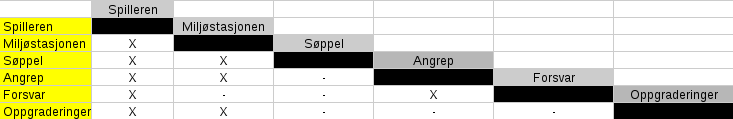
\includegraphics[scale=0.6]{images/spillmatrise.png}
\label{fig:spillmatrise}
\caption{Spillmatrise med de forskjellige elementene}
\end{figure}
\end{center}
I Figur~\cite{fig:spillmatrise} er elementene som interagerer er merket
med en \textbf{X} i den kollonnen og raden de elementene sammenfaller i.
Hvordan elementene interagerer er beskrevet nedenfor:
\begin{description}
\item \textbf{Spilleren}\\Spilleren sin oppgave er å samle søppel,
bygge våpen og forsvar, samt oppgradere miljøstasjonen.
\item \textbf{Miljøstasjonen}\\Miljøstasjonen tar imot og gjenvinner
søppelet. I tillegg er dette hovedbasen for spilleren, og står for alle
oppgraderingene. En miljøstasjon kan bli angrepet av andre spillere, og
interagerer derfor med våpen.
\item \textbf{Søppel}\\Blir plukket opp av spilleren, og lagt på
miljøstasjonen for gjenvinning.
\item \textbf{Angrep}\\Spillere kan angripe andre spillere sitt forsvar,
og miljøstasjonene deres.
\item \textbf{Forsvar}\\Forsvaret kan bli angrepet og ødelagt av våpen.
En spiller bygger forsvaret, derfor koblingen mellom spiller og forsvar.
\item \textbf{Oppgraderinger}\\Spilleren kan oppgradere miljøstasjonen
sin. Desse oppgraderingene baserer seg på statusen til miljøstasjonen.
\end{description}


% List all the elements that are directly related to or to the benefit
% of the player.

% Devise two sets of names for player elements. One set is a generic name
% (or code) and the other is its game name. 

% Describe the terminology that you use to describe the player’s
% properties.

%bruk ord: MILJØSTASJON, GJENVINNING. (ikke gjenvinningstasjon, utvinne, resirkulering)

\subsection{Elementer}
Dette avsnittet forteller om de forskjellige spillelementene som finnes
i Garbage Alert.
\subsubsection{Ressurser}
Ressurser er et viktig element i Garbage Alert. Ressursene er det som
gjør at spillere kan utvikle basen sin, bygge forsvar og utvikle angrep.
Valget av ressurser er basert på Mohs hardhetsskala av mineraler \cite{mohs}. Mohs hardhetskala er en liste over mineraler i rekkefølge etter absolutt hardhet, laget av geologen Friedrich Mohs. Hvert mineral skal kunne skrape mineralet som står foran på listen. Ressursene i Garbage Alert er ikke helt korrekte i forhold til Mohs hardhetsskala, men basert på denne. Idèen er at hver de seks ressursene i spillet følger samme regel, nemlig at den ene ressursen er hardere enn den andre og har mulighet til å ødelegge den. 
De forskjellige typene utvinnbare ressurser er:
\begin{description}
	\item \textbf{Papp}\\ Denne ressursen kan utvinnest uten å måtte
oppgradere miljøstasjonen. Dette er den enkleste ressursen å få fatt i,
men skaper kun relativt svake angrep/forsvar.
	\item \textbf{Plast}\\ Denne ressursen kan man utvinne etter å ha
oppgradert hovedbasen èn gang.
	\item \textbf{Tre}\\ Tre kan utvinnest dersom hovedbasen har blitt
oppgradert til dette. Tre er på samme oppgraderingsnivå som plast, med andre ord må
spilleren velge mellom desse to i begynnelsen. Tre er derimot hardere enn plast i dette spillet.
	\item \textbf{Jern}\\ Jern er mulig å utvinne dersom spilleren først
oppgraderer til tre.
	\item \textbf{Stål}\\ Stål bygger på at spilleren først har
oppgradert til plast.
	\item \textbf{Titan}\\ Titan er den siste ressursen som er mulig å
utvinne. For å kunne utvinne titan må spilleren først ha skaffet seg
alle utvinningsutvidelsene til hovedbasen.
\end{description}


Det er også mulig å skade forsvar/våpen som er bygget av en bedre ressurs enn våpenet. Dette er implementert slik at ingen våpen/forsvar blir uovervinnelige. Figur \ref{fig:ressursoppgraderinger} framstiller hvilke utvidelser man må ha for å kunne oppgradere til neste nivå. Allerede helt fra starten av spillet må man velge om man først vil oppgradere til tre, eller til plast (se seksjon \ref{miljostasjon}). 

	\begin{figure} [H]
				\begin{center}
					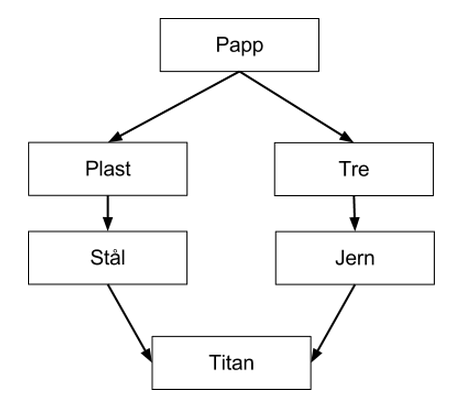
\includegraphics[scale=0.5]{images/oppgraderingstre}
				\end{center}
			\caption{Ressursoppgraderinger}
			\label{fig:ressursoppgraderinger}
	\end{figure}

\subsubsection{Ressursutvinning}
En spiller skaffer seg ressurser ved å gjenvinne søppel som ligger
spredt rundt på øya. Dette blir gjort ved hjelp av miljøstasjonen
som hver spiller starter med.
\subsubsection{Miljøstasjon} \label{miljostasjon}
Miljøstasjonen er det mest sentrale spillelementet i Garbage
Alert. Denne kan bli sett på som hovedbasen i spillet.
Miljøstasjonen kan oppgraderes på tre måter for å forbedre effektiviteten:\\
\begin{description}
	\item \textbf{Volum/Utvinningsgrad}\\Denne oppgraderingen kan øke utvinningsgraden og volumet av søppel som blir brukt i gjennvinningsprosessen. Restavfallet (søppelet som ikke blir gjenvunnet) vil på magisk vis bli borte. Tabell \ref{tab:effektivitet} viser oppgraderingene for Volum/Utvinningsgrad. Man starter på nivå 0, og deretter kan man oppgradere ett trinn ad gangen.
	\item \textbf{Buffer}\\Miljøstasjonen kan få en buffer hvor spilleren kan samle opp søppel, som automatiserer gjenvinningsprosessen til en viss grad. Dermed kan spilleren bruke mindre tid på å sørge for at søppelet på øyen blir flyttet til miljøstasjonen.
	\item \textbf{Ressurser}\\For å kunne gjenvinne nye typer ressurser må
		spilleren oppgradere gjenvinningsstasjonen. Her får spilleren valget
		mellom to ulike veier som vil avgjøre hvilke ressurser spilleren får
		tilgang til (se figur \ref{fig:ressursoppgraderinger}).
\end{description}

\begin{table} \label{tab:effektivitet}
\begin{tabular}[\textwidth]{ l  l  p{3cm}  l  p{4cm} } %\label{tab:effektivitet}
\hline
\bf{Effektivitet} & \bf{Utvinningsgrad} & \bf{Volum} & \bf{Tid} & \bf{Ressurskrav} \\
\hline
Nivå 0 & 10 & 10 & 15sek & Ingen  \\
Nivå 1 & 20 & 10 & 15sek & Papp \\
Nivå 2 & 30 & 10 & 15sek & Papp, og plast eller tre \\
Nivå 3 & 30 & 20 & 15sek & Papp, plast, tre, stål, jern og titan \\
\hline
\end{tabular}
\caption{Oppgraderinger for Volum/Utvinningsgrad}
\end{table}




\subsubsection{Forsvar}
Spillere kan bygge forsvar rundt øya si. Dette forsvaret vil forhindre
motspillere å angripe gjenvinningsstasjonen. Det vil finnes ulike typer
forsvarsmurer, som er kraftige/svake mot ulike typer angrep.
\subsubsection{Angrep}
En spiller får utdelt tre angrepsplattformer. På desse tre platformene
kan spilleren velge hvilke angrep han vil utvikle, basert på hvilke
tilgjengelige ressurser han har.
\subsubsection{Oppgraderinger}
Spilleren har mulighet til å oppgradere både gjenvinningsstasjonen,
våpen og forsvar. Hver type våpen og forsvar har tre nivå, der øking i
nivå vil gi hhv. kraftigere angrep og sterkere forsvar. De tre
våpenplassene på øya kan ha inneholde ulike våpen som kan oppgraderes
hver for seg.
Eksempel på forsvarsoppgradering:\\
Tremur (nivå 1) -> Tremur (nivå 2) -> Tremur (nivå 3).
\begin{quote}
Bør restruktureres!!\\
Spilleren kan utvinne ressurser ved å "dra" søppelenheter fra
forskjellige plasser på øya inn til gjennvinningsstasjonen. Hvilke
ressurser, og mengden av hver ressurs, som spilleren får ut fra en
enkelt søppelenhet er avhengig av nivået på gjennvinningsstasjonen og
hvilke typer oppgraderinger som er gjort. Spilleren kan også bruke sine
våpen til å bli kvitt søppelenheter. Her vil ubehandlede søppelenheter
kunne skytes på motstandere. Effekten av angrepet avhenger av spillerens
våpen, oppgraderingsnivå på våpenet og motstanderens forsvar. For å
beskytte seg mot angrep kan spilleren bygge mur rundt sin øy. Hvilke
våpen og forsvarsmurer som spilleren kan bygge er avhengig av hvilke
ressurser gjenvinningsstasjonen er i stand til å utvinne. Dette betyr at
valg av typer oppgradering for gjenvinningsstasjonen vil være avgjørende
for utviklingen av spillet.\\
\end{quote}

% Make a list of all objects that affect the player in a positive way.
% (i.e. health replenished)

% Define these objects by describing what affect they cause and how the
% player can use the object.
\subsection{Spillerpremier}

Gjennom å oppgradere ens miljøstasjon vil en kunne visuelt se at øya blir renere, atmosfæren blir klarere og bakgrunnsmusikken blir penere. Lystige lydeffekter signaliserer at en gjør noe som gir spilleren en fordel i forhold til motspillerne, for eksempel når en oppgraderer ens utstyr eller utfører et vellykket angrep mot sine motstandere. Dette håper vi skaper en positiv følelse av mestring hos spilleren. 

Videre er der en intrisitt verdi i å vinne et spill over ens medspillere.

For å kunne underbygge spillets underliggende tematikk om miljøvennlighet vil naturen straffe spillerne om de er er for miljøuvennlige med naturkatastrofer.

På samme måte som at muntre lydeffekter underbygger gode handlinger gjort av spilleren, vil dystre lydeffekter signalisere negative hendelser. Dette kan for eksempel være i det en blir angrepet av motspillerne. 
% This is where a description of the user’s control of the game can be
%placed.

% It is also recommended to think about which buttons on a device would
% be best suited for the game.

% Consider what the worst layout is, then ask you self if your UI is it
% still playable?

% A visual representation can be added, where we relate the physical
% controls to the actions in the game.


% TODO
% * Skrive om de svakeste elementene i grensesnittet
% * Referere til screenshots
% * Inkludere noe tekst om lydbildet?
% * Generell formattering, sammenslåing og sortering av avsnitt

\subsection{Brukergrensesnitt}



Brukergrensessnittet i spillet er i prototypen noe infantilt og uferdig.


Vi har bevisst valgt å holde språket i spillet norsk, og overalt hvor en finner tekst i spillet vil den være på norsk. % bah, møkkasetning.


Det en først ser når en starter spillet er en introskjerm som med sin grafikk og lydbilde er ment å sette spilleren i et kompetetivt sinnelag.

Fra denne skjermen er det mulig å starte spillet ved å trykke den store knappen markert "Start".
En mer ferdig versjon vil andre valg fra denne skjermen være å stille inn ting som spillernavn, samt mulighet for å koble flere spillere sammen i et flerspillerspill.


Spillets hovedskjerm % Forklare litt bedre hva vi mener med hovedskjerm
består av et overblikksbilde av alle øyer som er med i spillet. I prototypen er antallet begrenset til to, men en mer moden versjon vil inneholde muligheten til å spille flere enn to stykker samtidig. En skiller mellom en selv og andre ved bruk av ulike farger på spillernes miljøstasjon, våpen og forsvar. I prototypen har vi valgt å fargelegge de to faksjonene rød og blå.

I prototypen er denne skjermen et statisk fugleperspektiv av alle øyene og alle spillets elementer. En ferdig versjon vil og inneholde muligheten til å veksle mellom et detaljbilde av ens egen øy og overblikksbildet over alle øyer. Hvorvidt dette vil gjøres via en knapp som veksler mellom de to visningsmodi eller om en vil "klype for å zoome" er på dette stadiet uvisst og bør testes via brukertesting for å finne den optimale metoden.


Garbage Alert er tenkt å først og fremst spilles på mobiltelefoner og andre enheter med berøringsskjerm. En interagerer derfor med elementene på skjermen ved å trykke på de. Det en må være spesielt oppmerksom på med slike skjermer er å holde knapper store nok, samt at aller elementer på skjermen må være forskjellige nok til at det er enkelt å skille de fra hverandre på små skjermer.

Spillet kan og spilles på en datamaskin i en nettleser, og en kan derfor også bruke en musepeker for å trykke på elementene på samme måte.


Merk at da vi under utviklingen kun har testet prototypen på en dataskjerm er ikke spillet per nå tilpasset mobiltelefoner i så stor grad som det burde være. Enkle tester på mobiltelefon har dog blitt gjort, men har vært nedprioritert grunnet tidspress.

